\def\year{2015}
%File: formatting-instruction.tex
\documentclass[letterpaper]{article}
\usepackage{aaai16}
\usepackage{times}
\usepackage{helvet}
\usepackage{courier}
\usepackage{graphicx}
\usepackage{cleveref}
\frenchspacing
\setlength{\pdfpagewidth}{8.5in}
\setlength{\pdfpageheight}{11in}
\pdfinfo{
/Title (Human-Robot Collaboration: Affective Motivational Collaboration Theory)
/Author (Mahni Shayganfar, Charles Rich, Candace Sidner)}
\setcounter{secnumdepth}{0}
 \begin{document}
% The file aaai.sty is the style file for AAAI Press 
% proceedings, working notes, and technical reports.
%
\title{Human-Robot Collaboration: Affective Motivational Collaboration Theory}
\author{Mahni Shayganfar, Charles Rich, Candace Sidner\\
Worcester Polytechnic Institute\\
Fuller Laboratories, 100 Institute Road\\
Worcester, Massachusetts, 01609\\
}
\maketitle
\begin{abstract}
\begin{quote}
The capability of collaboration is critical in the design of symbiotic cognitive
systems. To obtain this functional capability, a cognitive system should possess
evaluative and communicative processes. Emotions and their underlying processes
provide such functions in social and collaborative environments. We investigate
the mutual influence of affective and collaboration processes in a cognitive
theory to support the interaction between humans and robots or virtual agents.
We develop new algorithms for these processes, as well as a new overall
computational model for implementing collaborative robots and agents. We build
primarily on the \textit{cognitive appraisal} theory of emotions and the
\textit{SharedPlans} theory of collaboration to investigate the structure,
fundamental processes and functions of emotions in a collaboration context.
\end{quote}
\end{abstract}

Intelligence is a set of mental abilities that enables a human to comprehend,
reason and adapt in the environment, and as a result, act effectively and
purposefully in that environment. Emotions play a crucial role in humans'
explanation of intelligent behaviors. Emotions affect not only what people do,
but also the way they do it \cite{cowie:concepts-definitions}. Sousa in The
Rationality of Emotion (\citeyear{sousa:rationality-emotion}) makes a case for
claiming that humans are capable of rationality largely because they are
creatures with emotions. Emotions significantly impact different procedures of
goal management, and action generation, execution, control, and interpretation
\cite{zhu:emotion-action}. Emotions are dynamic episodes that not only make
changes in cognitive states, but also produce a sequence of response patterns on
one's verbal and nonverbal behaviors \cite{scherer:expression-appraisal}.
Emotions typically occur in response to an event, usually a social event, real,
remembered, anticipated, or imagined. They are associated with distinctive
relational meanings with the individual's experiences and environment
\cite{parkinson:holds-emotion}. Emotions are evaluative and responsive patterns
that serve the function of providing appraisal about whether the ongoing event
is harmful or beneficial for the well-being of an individual
\cite{zhu:emotion-action}. Therefore, reasoning and emotional processes have an
integral and a supportive relationship, rather than a conflicting one.

The idea of having robots or other intelligent agents living in a human
environment has been a persistent dream from science fiction books to artificial
intelligence and robotics laboratories. However, there are many challenges in
achieving collaboration between robots and humans in the same environment. Some
of these challenges involve physical requirements, some involve cognitive
requirements, and some involve social requirements. Thus far, there has been an
emphasis on the design of robots to deal with the physical requirements. Many
researchers are also working on the cognitive requirements, inspired by a
diverse set of disciplines
\cite{laird:soar,scheutz:integration-cognition,hemion:cognition-building-blocks}.
As time passes, there is an increasing recognition of the importance of the social
requirements, and how cognitive systems can include the influence of others.

\subsection{Social Functions of Emotions}

Emotions describe interpersonal dynamics in a way that they can constitute
individuals' relationships \cite{parkinson:emotions-social,tiedens:social-life}.
Humans are able to communicate their emotions in a social context. The social
functions of emotions are the reason behind why humans try to communicate their
emotions. One aspect of expressing
and communicating emotion in a social context is to express one's social motives
and intentions \cite{hess:darwin-emotion}. Another aspect of communicating
emotions is to reveal the underlying mental states of an individual
\cite{parkinson:emotion-communication}. In
(\citeyear{kleef:emotion-regulate-social}) Van Kleef has discussed the idea of
inferential processes with which individuals can infer information about others'
feelings, relational orientations and behavioral intentions based on their
emotional expressions. He also argues that emotional expressions can impact
social interactions by eliciting others' affective responses.

\section{Motivation}

Functional coexistence is an important aspect of the symbiotic cognitive
systems in social environments. Collaboration requires coexistence with
the others and describes how a cognitive agent can function in such environment.
Therefore, the ability to collaborate with humans in the same environment is
crucial for cognitive agents. In fact, a cognitive agent's ability to understand
the collaborative environment impacts the effectiveness of a collaboration.
Examples of cognitive capabilities that support the effectiveness of
collaboration include: a) perceiving one's own internal states and b)
communicating them, c) coordinating personal and group behaviors, d) identifying
self and mutual interests, e) recognizing the accountability of private and
shared goals, f) selecting appropriate actions with respect to events, and g)
engaging others in collaboration.

We are investigating the cognitive processes involved in a collaboration in the
context of a cognitive architecture. There are several well-developed cognitive
architectures, e.g., Soar \cite{laird:soar} and ACT-R \cite{anderson:act-r},
each with different approaches to defining the basic cognitive and perceptual
operations. There have also been efforts to integrate affect into these
architectures \cite{dancy:actR-physiology-affect,marinier:behavior-emotion}. In
general, however, these cognitive architectures do not focus on processes to
specifically produce emotion-regulated goal-driven collaborative behaviors. At
the same time, existing collaboration theories, e.g., SharedPlans theory
\cite{grosz:plans-discourse}, focus on describing the structure of a
collaboration in terms of fundamental mental states, e.g., mutual beliefs or
intentions. However, they do not describe the associated processes, their
relationships, and their influences on each other. In contrast,
\textit{Affective Motivational Collaboration Theory} deals with the major
processes, including affective and motivational processes, having an impact on
the collaboration structure. This theory is informed by research in psychology
and artificial intelligence. Our contribution, generally speaking, will be to
synthesize prior work on motivation, appraisal and collaboration, and thus to
provide a new theory which describes the prominent emotion-regulated goal-driven
phenomena in a dyadic collaboration.

\section{Affect and Collaboration}

Collaboration is a coordinated activity in which the participants work jointly
to satisfy a shared goal \cite{grosz:plans-discourse}. There are many important
unanswered questions about the involvement of an individual's cognitive
abilities during collaboration. Some of these questions are related to the
dynamics of collaboration, as well as the underlying mechanisms and processes.
For instance, a general mechanism has yet to be developed that allows an agent
to initiate proactive collaborative behaviors when it faces a blocked task.
There is also a lack of a general mechanism that, in the event of a task
failure, allows an agent to consider the collaborator's anticipated mental
states and emotions, while managing its own internal goals and the
collaboration's shared goal. There are also other questions about the components
involved in these processes at the cognitive level, such as the processes that
are involved for evaluative, regulatory or motivative purposes. There has also
not been enough attention on the processes that are involved to maintain the
social aspects of a collaboration.

Emotions have a key role in influencing the cognitive processes involved in
social interaction and collaboration. Emotion processing and decision-making are
integral aspects of daily life and maintain their prominence during social
interaction and collaboration. However, researchers' understanding of the
interaction between emotions and collaborative behaviors is limited. We believe
that the evaluative role of emotions, as a part of cognitive processes, helps an
agent to perform appropriate behaviors during a collaboration. To work jointly
in a coordinated activity, participants (collaborators) act based on their own
understanding of the world and the anticipated mental states of the counterpart;
this understanding is reflected in their collaborative behaviors. Emotions are
pivotal in the collaboration context, since their regulatory and motivational
roles enhance an individual's autonomy and adaptation as well as his/her
coordination and communication competencies in a dynamic, uncertain and
resource-limited environment.

\section{Affective Motivational Collaboration Theory}

We are building Affective Motivational Collaboration Theory on the foundations
of the \textit{SharedPlans} theory of collaboration \cite{grosz:plans-discourse}
and the \textit{cognitive appraisal} theory of emotions
\cite{gratch:domain-independent}. Affective Motivational Collaboration Theory is
about the interpretation and prediction of observable behaviors in a dyadic
collaborative interaction. The theory focuses on the processes regulated by
emotional states. The observable behaviors represent the outcome of reactive and
deliberative processes related to the interpretation of the self's relationship
to the collaborative environment. 

Affective Motivational Collaboration Theory aims to explain both rapid emotional
reactions to events as well as slower, more deliberative responses. The reactive
and deliberative processes are triggered by two types of events:
\textit{external} events, such as the other's \textit{utterances} and
\textit{primitive actions}, and \textit{internal} events, comprising changes in
the self's mental states, such as belief formation and emotional changes.
Affective Motivational Collaboration Theory explains how emotions regulate the
underlying processes when these events occur during collaboration. This theory
elucidates the role of motives as goal-driven emotion-regulated constructs with
which an agent can form new intentions to cope with internal and external
events. Affective Motivational Collaboration Theory explains the functions of
emotions in a dyadic collaboration and show how affective mechanisms can
coordinate social interactions by enabling one to anticipate other's emotions,
beliefs and intentions.

Our focus is on the mechanisms depicted as mental processes in Figure
\ref{fig:cpm} along with the mental states. The \textit{Mental States} includes
self's (robot's) beliefs, intentions, motives, goals and emotion instances as
well as the anticipated Mental States of the other (human). \textit{Beliefs} are
a crucial part of the Mental States. Beliefs can be generated based on whether
they are shared or not between the collaborators. The SharedPlans
\cite{grosz:shared-plans,grosz:plans-discourse} theory is the foundation of this
view on beliefs in which for any given proposition the agent may have: a)
private beliefs (the agent believes the human does not know these), b) the
inferred beliefs of the human (the agent believes the human collaborator has
these beliefs), and c) mutual beliefs (the agent believes both the self and the
human have these same beliefs and both of them believe that). Beliefs also can
be generated based on who or what they are about, i.e., beliefs can be about the
self, the other, or they can be about the environment. \textit{Intentions} are
mental constructs directed at future actions. They play an essential role in
taking actions according to the collaboration plan, and behavior selection in
the Coping mechanism. \textit{Goals} help the agent to create and update its
collaboration plan according to the current private and shared goal content and
structure. Goals direct the formation of intentions to take appropriate
corresponding actions during collaboration. Goals also drive the Motivation
mechanism to generate required motive(s) in uncertain or ambiguous situations,
e.g., to minimize the risk of impasse or to reprioritize goals. Therefore,
\textit{motives} as an additional mental construct are required. Motives are
mental constructs which can initiate, direct and maintain goal-directed
behaviors. They are created by the emotion-regulated Motivation mechanism.
Motives can cause the formation of a new intention for the agent according to:
a) its own emotional states (how the agent feels about something), b) its own
private goal (how an action helps the agent to make progress), c) the
collaboration goal (how an action helps to achieve the shared goal), and d)
other's anticipated beliefs (how an action helps the other). \textit{Emotions}
in Mental States are emotion instances that are elicited by the Appraisal
mechanism.

\vspace*{-2mm}
\begin{figure}[tbh]
  \centering
  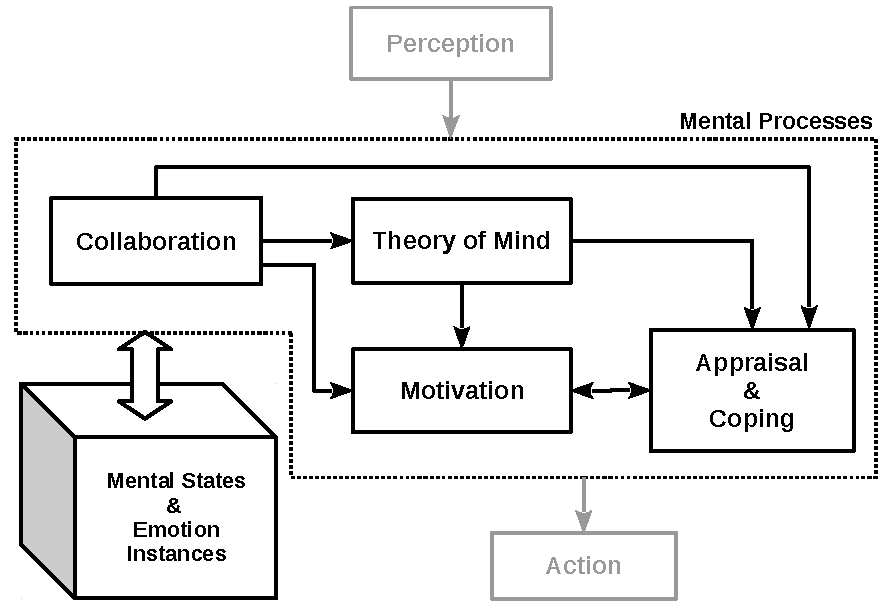
\includegraphics[width=0.474\textwidth]{figure/theory-general-croped.pdf}
  \caption{Computational framework based on Affective Motivational Collaboration
  Theory (arrows indicate primary influences between mechanisms).}
  \label{fig:cpm}
  \vspace*{-2mm}
\end{figure}

The \textit{Collaboration} mechanism maintains constraints on actions, including
task states and the ordering of tasks. The Collaboration mechanism constructs a
hierarchy of tasks and also manages and maintains the constraints and other
details of the collaboration specified by the plan. These details include the
\textit{inputs} and \textit{outputs} of individual tasks, the
\textit{preconditions} specifying whether it is appropriate to perform a task,
and the \textit{postconditions} specifying whether a just-completed task was
successful (which can be used as an indication of an impasse or failure).
Collaboration also keeps track of the focus of attention, which determines the
salient objects, properties and relations at each point of the collaboration.
Moreover, Collaboration mechanism has the ability to shift the focus of
attention during the collaboration. The Collaboration mechanism also provides
processes to update and monitor the shared plan.
  
\textit{Appraisal} is a subjective evaluation mechanism based on individual
processes each of which computes the value of the appraisal variables used in
our computational model. The Appraisal mechanism is responsible for evaluating
changes in the self's Mental States, and the state of the collaboration
environment. The Collaboration mechanism needs the evaluative assistance of the
Appraisal mechanism for various reasons. The course of a collaboration is based
on a full or a partial plan which needs to be updated as time passes and
collaborators achieve, fail at or abandon a task assigned to them. The failure
of a task should not destroy the entire collaboration. Appraising the
environment and the current events helps the agent to update the collaboration
plan and avoid further critical failures during collaboration. 

Appraisal and collaboration structure have reciprocal influences on each
other. We use collaboration structure to compute appraisal variables, i.e.
relevance, desirability, expectedness, and controllability, for every event.
Mutually, we use appraisals to regulate the goal management process during
collaboration. By using reverse appraisal \cite{gratch:reverse-appraisal} of the
human collaborator's emotion, and its own appraisal of individual goals, the
robot is able to successfully shift the focus of attention from the blocked goal
(causing to elicit negative emotions, e.g., worry) to an appropriate one to
maintain the collaboration. Goal management is one of the crucial reciprocal
influences of appraisal on a collaboration structure. We also investigate how
appraisal impacts forming new motives as well as the action selection process.
Therefore, in order to collaborate successfully, a collaborative robot should
possess an adaptation mechanism to update the shared plan, and adopt
affect-regulated goal-driven motives while being able to choose appropriate
actions.

The \textit{Coping} mechanism is responsible for interpreting ongoing changes
in the Mental States and adopting the appropriate behavior with respect to these
changes. The Coping mechanism provides the self with different coping strategies
associated with changes in the self's mental states with respect to the state of
the collaboration.

The \textit{Motivation} mechanism coordinates with the Appraisal mechanism. The
purpose of this component is to generate new motives. These motives are
generated based on what the agent believes about the environment including self
and the other collaborator and the corresponding appraisals. The agent uses
these motives to achieve a private or shared goal according to new conditions,
to interact better with a human who needs social interactions, or to evaluate
the success of task performances. The Motivation mechanism operates whenever the
self a) requires and intends to take a new action, b) requires a new motive to
overcome an internal impasse in an ongoing task, or c) wants to provide an
external motive to the other based on other's model when the other faces a
problem in a task.

The agent uses the \textit{Theory of Mind} mechanism to infer and attribute
beliefs, intentions, motives and goals to its collaborator based on the user
model it creates and maintains during the course of the collaboration. In
other words, the Theory of Mind mechanism is the mechanism that infers a model
of the other's anticipated mental state. The self progressively updates this
model during the collaboration.

\section{Conclusion}

The capability of collaboration is crucial in symbiotic cognitive systems. The
nature of coexistence requires the ability to work together, in the same
environment. To successfully work together symbiotic cognitive systems need to
be able to a) communicate and understand social communication, and b)
collaborate and maintain a collaborative structure. Emotions have a crucial role
in communicating one's mental state, motivating one's actions, and evaluating
and interpreting one's internal states and the environment. Emotion functions
are important because not only they regulate one's internal processes, but they
also provide social characteristics that the self needs to manifest its
collaborative behavior. Therefore, the integration of emotion-regulated
processes, e.g., appraisal, and collaboration structure and its underlying
processes can lead us to a more functionally capable symbiotic cognitive system.
Affective Motivational Collaboration Theory is a computational theory which
provides emotion-regulated goal-driven mechanisms for a colaborative robot. This
theory, combines emotion-based processes, such as appraisal and coping, with
collaboration processes, such as planning, in a single unified framework.

\section*{Acknowledgments}
This work is supported by the National Science Foundation under award
IIS-1012083. Any opinions, findings, and conclusions expressed in this material
are those of the authors and do not necessarily reflect the views of the
National Science Foundation.

\bibliography{mshayganfar.bib}
\bibliographystyle{aaai}

\end{document}
